% Options for packages loaded elsewhere
\PassOptionsToPackage{unicode}{hyperref}
\PassOptionsToPackage{hyphens}{url}
\documentclass[
  11pt,
]{article}
\usepackage{xcolor}
\usepackage[margin=1in]{geometry}
\usepackage{amsmath,amssymb}
\usepackage{iftex}
\ifPDFTeX
  \usepackage[T1]{fontenc}
  \usepackage[utf8]{inputenc}
  \usepackage{textcomp} % provide euro and other symbols
\else % if luatex or xetex
  \usepackage{unicode-math} % this also loads fontspec
  \defaultfontfeatures{Scale=MatchLowercase}
  \defaultfontfeatures[\rmfamily]{Ligatures=TeX,Scale=1}
\fi
% Typography: Palatino for body + matching math, Helvetica for sans, beraMono for tt.
\usepackage{mathpazo}
\usepackage[scaled=0.92]{helvet}
\usepackage[scaled=0.85]{beramono}
% Section heading style + line spacing + headers + sub-caption font.
\usepackage{titlesec}
\titleformat{\section}{\Large\bfseries\sffamily}{\thesection}{0.6em}{}
\titleformat{\subsection}{\large\bfseries\sffamily}{\thesubsection}{0.5em}{}
\titleformat{\subsubsection}{\normalsize\bfseries\sffamily}{\thesubsubsection}{0.5em}{}
\usepackage{setspace}\setstretch{1.15}
\usepackage{fancyhdr}\pagestyle{fancy}\fancyhf{}
\fancyhead[L]{\small\textit{Cole \textbar{} Probing Geneformer scaling}}
\fancyhead[R]{\small\thepage}
\renewcommand{\headrulewidth}{0.4pt}
\usepackage[font={small},labelfont={bf,sf}]{caption}
\ifPDFTeX\else
  % xetex/luatex font selection
\fi
% Use upquote if available, for straight quotes in verbatim environments
\IfFileExists{upquote.sty}{\usepackage{upquote}}{}
\IfFileExists{microtype.sty}{% use microtype if available
  \usepackage[]{microtype}
  \UseMicrotypeSet[protrusion]{basicmath} % disable protrusion for tt fonts
}{}
\makeatletter
\@ifundefined{KOMAClassName}{% if non-KOMA class
  \IfFileExists{parskip.sty}{%
    \usepackage{parskip}
  }{% else
    \setlength{\parindent}{0pt}
    \setlength{\parskip}{6pt plus 2pt minus 1pt}}
}{% if KOMA class
  \KOMAoptions{parskip=half}}
\makeatother
\setlength{\emergencystretch}{3em} % prevent overfull lines
\providecommand{\tightlist}{%
  \setlength{\itemsep}{0pt}\setlength{\parskip}{0pt}}
\usepackage{bookmark}
\IfFileExists{xurl.sty}{\usepackage{xurl}}{} % add URL line breaks if available
\urlstyle{same}
\hypersetup{
  colorlinks=true,
  citecolor={blue!50!black},
  urlcolor={blue!50!black},
  linkcolor={blue!50!black},
  pdfcreator={LaTeX}}
\usepackage[round,authoryear]{natbib}
\usepackage{graphicx}

\title{What scale buys for single-cell foundation models: \\[2pt]
\large a controlled probe of Geneformer V1, V2-104M, and V2-316M}
\author{William Cole \\[2pt]
{\small Baltimore AI, Baltimore, MD, USA} \\
{\small\texttt{info@baltimoreai.org} \,\textbar\, ORCID \href{https://orcid.org/0009-0004-0578-9853}{0009-0004-0578-9853}}}
\date{6 May 2026}

\begin{document}

\maketitle

\begin{center}\small\itshape Project: \textbf{Morpheus}. Preprint v1, 6 May 2026.\end{center}
\begin{abstract}
\noindent We probe whether Geneformer's frozen single-cell representations encode
known regulatory structure, using donor-stratified linear probes on
100,000 healthy human blood/immune cells (CELLxGENE Census) across three
pretrained variants: V1-10M (Genecorpus-30M), V2-104M and V2-316M (both
pretrained on \textasciitilde104M cells). Three probes: cell-type
identity (L1), TF$\to$target structure (L2, expression-matched negatives),
and hub-TF identity (L3, top-decile out-degree in DoRothEA $\cup$ CollecTRI).
All comparisons include a label-permutation selectivity control \citep{hewitt2019} and a bag-of-genes baseline. The within-V2 family forms
our only clean parameter-scaling axis.

\textbf{Three findings.} (1) \textbf{Hub-TF identity is encoded at the
smallest variant} (V1-10M, AUC 0.72) and exceeds the bag-of-genes
baseline by approximately +0.20 AUC at every scale (V1 +0.22 {[}+0.13, +0.29{]}, V2-104M +0.21 {[}+0.14, +0.27{]}, V2-316M +0.20 {[}+0.13, +0.27{]}) --- a gap that survives a random-initialization control at
matched embedding dimensionality (random-init AUC 0.42 at 256d, 0.53 at 768d, 0.44 at 1152d), ruling out the alternative that the signal is
geometric room rather than learned structure. (2) \textbf{TF$\to$target
probe gains are large and selectivity-passing across V1$\to$V2 (+0.054 AUC,
p=10$^{-16}$, n=375 TFs) but do not improve under pure parameter scaling
within V2} (V2-316M $-$ V2-104M $\Delta$=$-$0.003 {[}$-$0.014, +0.008{]}, p=0.45).
The V1$\to$V2 gain is therefore not separable from pretraining-corpus
expansion. (3) \textbf{Cell-type identity (L1) shows no measurable
improvement under pure parameter scaling} (V2-316M $-$ V2-104M $\Delta$=$-$0.007
{[}$-$0.034, +0.017{]}); V2-316M fails to exceed the bag-of-genes baseline
($\Delta$=+0.019 {[}$-$0.001, +0.043{]}, p=0.31; we report this as ``fails to
reject,'' not ``matches,'' because we did not perform formal equivalence
testing).

The contribution is methodological as much as empirical: scaling claims
for single-cell foundation models that compare across model-family
transitions confound parameter count with pretraining-corpus and
vocabulary changes, and the only clean within-family parameter-scaling
axis available to us shows no measurable gain on any probe.

\end{abstract}

\section{Introduction}\label{introduction}

Single-cell foundation models (scFMs) train large transformers on tens
to hundreds of millions of single-cell transcriptomes with the promise
that the resulting representations will encode biological structure
useful across many downstream tasks. Geneformer \citep{theodoris2023},
scGPT \citep{cui2024}, scFoundation \citep{hao2024scfoundation}, and Nicheformer
\citep{schaar2025nicheformer} are the canonical instances of this paradigm. Each
ships a frozen embedding that practitioners use as a feature extractor
for cell-type classification, batch integration, perturbation
prediction, and gene-regulatory inference. The implicit claim is
twofold: that pretraining at scale writes biologically meaningful
structure into the parameter space, and that more pretraining --- more
cells, more parameters, larger vocabularies --- writes more of it.
Neither half of that claim has been straightforward to verify.

The empirical case for scFM scale is becoming more guarded. \citet{boiarsky2025} benchmark six scFMs against simple baselines and find that
the relative ranking is task- and tissue-dependent, with raw expression
baselines competitive on several integration metrics. \citet{kedzierska2025} report that zero-shot evaluation reveals ``reliability
challenges'' for scGPT and Geneformer that simpler methods do not
exhibit. \citet{ahlmanneltze2025perturbation} show that on
perturbation-effect prediction --- a task scFMs were explicitly designed
to address --- none of the six models tested consistently beats an
additive linear baseline. The pattern across these papers is not that
scFMs are useless; it is that the gap between scFM embeddings and
stubborn classical baselines is smaller, and more task-contingent, than
the original model papers implied.

A separate question, mostly unasked in the scFM literature, is what
\emph{kind} of scaling produces the apparent gains. In large language
models the analogous question is well posed: \citet{kaplan2020scaling}
established that loss scales as a power-law in parameter count, dataset
size, and compute over many orders of magnitude, and \citet{hoffmann2022chinchilla} --- the Chinchilla paper --- showed that compute-optimal
training requires scaling parameters and tokens jointly, so that ``more
parameters at fixed data'' is generically sub-optimal. The Chinchilla
result reframes any pre-Chinchilla scaling claim that increased only one
axis: the gain attributed to parameters was partly a gain from the data
scaling that came along for the ride. The same confound is present, in
starker form, in the scFM literature. The Geneformer release adds a V2
family at 104M and 316M parameters trained on a fresh
\textasciitilde104M-cell corpus with a new vocabulary; the V1 family at
10M parameters was trained on Genecorpus-30M with a different
vocabulary. A V1-vs-V2 comparison conflates parameter count,
pretraining-corpus size, and vocabulary in a single step. The only clean
parameter-scaling axis the public Geneformer checkpoints offer is
V2-104M $\to$ V2-316M (3$\times$ parameters, fixed corpus, fixed vocabulary).
Neither the original Geneformer paper nor the recent Theodoris-group
scaling paper \citep{venkatesh2026} isolates this axis on frozen
embeddings.

Probing --- training a simple supervised classifier on top of frozen
representations to ask whether a target property is linearly recoverable
--- is the natural tool for this question. The methodology has a clean
lineage in NLP: \citet{alainbengio2016probes} introduced linear
classifier probes for intermediate-layer analysis; \citet{conneau2018}
made probing canonical for sentence embeddings; \citet{hewitt2019}
introduced the selectivity control (a probe that succeeds on the real
task must fail on a randomized control task) that distinguishes ``the
property is in the embedding'' from ``the probe is expressive enough to
memorize anything''; \citet{belinkov2022} reviews the failure modes that an
unaudited probing study runs into. Despite this provenance, scFM
evaluation rarely couples probing with the full set of controls ---
random-initialization, label-permutation selectivity, and a non-trivial
expression-level baseline --- that the NLP probing literature has
settled on as a minimum.

In this paper we ask, on a single donor-stratified human blood/immune
cohort of 100,000 cells, three probing questions of three Geneformer
variants (V1-10M, V2-104M, V2-316M): does the frozen embedding recover
(i) cell-type identity at the level of CL-ontology labels, (ii)
TF$\to$target gene-regulatory edges, and (iii) the identity of
high-out-degree hub transcription factors. Each comparison is paired
with a bag-of-genes baseline, a random-initialization control at matched
embedding dimensionality, and a Hewitt-Liang label-permutation
selectivity control. We make four contributions. First, we show that
hub-TF identity is encoded in Geneformer's input gene-token embeddings
at the smallest tested variant (V1-10M, AUC 0.72) and exceeds
bag-of-genes by +0.20 AUC at every scale, with a gap that survives the
random-initialization control at matched dimensionality --- ruling out
the ``geometric room'' alternative. Second, we show that the large V1$\to$V2
gain on TF$\to$target structure (+0.054 AUC, p=10$^{-16}$) is not separable from
the pretraining-corpus and vocabulary expansion that accompany the V1$\to$V2
transition, and that the only clean parameter-scaling axis available to
us (V2-104M $\to$ V2-316M) shows no measurable gain. Third, we show that on
cell-type identity Geneformer's largest publicly available variant fails
to exceed the bag-of-genes baseline ($\Delta$=+0.019, p=0.31; we report this as
``fails to reject'' rather than ``matches'' because we do not perform
formal equivalence testing). Fourth, by isolating the parameter-only
axis from the corpus-expansion axis, we show that for Geneformer
specifically the apparent ``gains from scale'' in V1-vs-V2 comparisons
are concentrated in the corpus axis rather than the parameter axis ---
the single-cell analog of the Chinchilla observation that pure parameter
scaling at fixed data is the wrong axis to push.

\section{Methods}\label{methods}

\subsection{Data acquisition}\label{data-acquisition}

We assembled a single-tissue, single-condition cell corpus from the CZ
CELLxGENE Discover Census \citep{cellxgene2025}, accessed through the \texttt{cellxgene\_census}
Python client. The Census query restricted cells to
\texttt{tissue\_general\ ==\ "blood"}, \texttt{disease\ ==\ "normal"},
\texttt{is\_primary\_data\ ==\ True}, and one of four 10x Genomics
assays (3' v2, 3' v3, 5' v1, 5' v2); restricting to a single tissue and
to healthy donors removes two of the largest sources of biological
variance that would otherwise confound a probe of representational
structure. Donor-stratified sampling was performed in two phases: we
first pulled the obs metadata only, ordered donors by random shuffle
(seed 0), and admitted donors whole into the working set in order until
the cumulative cell count first reached the 100,000-cell target; only
the single boundary donor was randomly subsampled to bring the total to
exactly 100,000 cells. This procedure preserves the within-donor cell
distribution for every donor except the boundary case and is a
prerequisite for the donor-stratified cross-validation described below.
The final corpus comprised 100,000 cells from 15 donors, 41 datasets,
and 71 distinct cell types annotated against the Cell Ontology \citep{diehl2016cellontology}.

Counts were normalized per cell to a target sum of 10,000 and
\texttt{log1p}-transformed using \texttt{scanpy} \citep{wolf2018scanpy}. We
chose \texttt{log1p(CP10K)} over more elaborate transformations (e.g.,
scran pooling, residual transformations) on the basis of
\citet{ahlmanneltze2023normalization}, who benchmarked four classes of single-cell
normalization and reported that \texttt{log1p} followed by PCA performs
as well as or better than more sophisticated alternatives across a range
of downstream tasks. Geneformer's rank-value tokenizer expects raw
CP10K, so the embedding-extraction code reconstructs CP10K via
\texttt{expm1} of the cached log-normalized matrix; this round trip is
exact in float32. The cached corpus was stored as a sparse CSR
\texttt{.h5ad} keyed by Ensembl gene ID, with stable per-cell
identifiers carried through every downstream artifact.

The transcription-factor regulon was assembled by unioning DoRothEA
confidence levels A, B, and C \citep{garciaalonso2019dorothea} with CollecTRI \citep{mullerdott2023collectri}, both pulled through the
\texttt{decoupler} Python package \citep{badiaimompel2022decoupler}. After
resolving HGNC symbols to Ensembl IDs through a union of the Geneformer
gc30M and gc104M gene-name dictionaries (later releases winning on
collision), the regulon contained 73,269 directed TF$\to$target edges across
1,194 unique TFs. Critically, we did not apply a model-vocabulary filter
to this edge file. Per-model vocabulary restriction happens at probe
time through each model's gene index, which guarantees that V1 and V2
probes evaluate against the same canonical edge set rather than against
differently filtered subsets.

\subsection{Donor-stratified cross-validation}\label{donor-stratified-cross-validation}

We partitioned cells into five cross-validation folds at the donor
level: every cell from a given donor is assigned to exactly one fold.
Folds were constructed by greedy bin-packing (donors processed
largest-first, each donor placed into the currently smallest fold), and
a runtime assertion verified that no donor crossed fold boundaries. The
audit passed for all 15 donors.

This protocol follows the principle articulated by
\citet{zimmerman2021pseudoreplication} that cells from a common donor are not independent
samples --- intra-donor expression correlations exceed inter-donor
correlations, producing inflated type-I error and over-optimistic
generalization estimates when within-donor cells are split across train
and test. Although those authors proposed mixed-effects models for
differential expression rather than a cross-validation scheme, the
underlying non-independence applies identically to probing. We therefore
depart from the convention established in the most-cited automatic
cell-identification benchmark in scRNA-seq \citep{abdelaal2019},
which stratifies folds by cell-type proportion only and permits
arbitrary donor leakage between train and test partitions. Published
cell-type-classification accuracies obtained under that convention are
not directly comparable to ours; our protocol is the more conservative
of the two.

\subsection{Model variants}\label{model-variants}

We extracted frozen embeddings from three pretrained Geneformer
checkpoints distributed by the original authors \citep{theodoris2023}. V1-10M comprises
approximately 10 million parameters in 6 transformer layers of width 256
and 4 attention heads per layer, with vocabulary size 25,424 (the
Genecorpus-30M, or ``gc30M'', dictionary). It was pretrained on
Genecorpus-30M (\textasciitilde30 million cells). V2-104M comprises
approximately 104 million parameters in 12 layers of width 768 with 12
heads, with vocabulary size 20,275 (the gc104M dictionary), pretrained
on a refreshed corpus of approximately 104 million cells. V2-316M
comprises approximately 316 million parameters in 18 layers of width
1,152 with 18 heads, sharing both the gc104M vocabulary and the V2
pretraining corpus.

Three changes co-occur across the V1$\to$V2 transition: parameter count (10$\times$
larger), pretraining-corpus size (\textasciitilde3.5$\times$ larger), and
vocabulary (gc30M $\to$ gc104M, with associated changes in tokenizer
median-expression statistics). The V1$\to$V2 step is therefore confounded as
a parameter-scaling experiment. The only clean parameter-scaling axis
available across publicly released Geneformer checkpoints is V2-104M $\to$
V2-316M, which holds pretraining corpus and vocabulary fixed and triples
parameter count. Every cross-variant comparison in this paper is
labelled explicitly as either ``confounded (V1$\to$V2)'' or ``parameter-only
(within V2)''.

\subsection{Embedding extraction}\label{embedding-extraction}

Cell embeddings were computed as the mean of the final-layer hidden
state across non-padding tokens, following the empirical finding by
\citet{reimers2019sbert} that mean-pooling over non-pad tokens yields
the strongest fixed-size sentence representation for downstream linear
probes among standard pooling schemes (CLS, max, mean). Inference used
\texttt{transformers} \citep{wolf2020transformers} and \texttt{torch} \citep{paszke2019pytorch} with weights frozen and gradients disabled. Tokenization
followed the published Geneformer rank-value scheme: per-cell expression
was median-scaled using each variant's gene-median dictionary, sorted in
descending order, truncated to the top 2,048 tokens, and dynamically
truncated within each batch to the longest non-pad sequence. The
pipeline streamed cells.h5ad in chunks of 2,000 cells, densifying only
the active chunk and writing pooled embeddings into a \texttt{numpy}
memmap; the full expression matrix is never materialized in dense form,
keeping peak memory below the 24 GB target on the laptop runs.

Gene embeddings were taken directly from the model's input
token-embedding lookup table
(\texttt{model.embeddings.word\_embeddings.weight}) rather than from any
contextualized aggregate. This isolates what pretraining writes into the
parameter space without per-batch confounds --- the same gene token
receives the same vector regardless of its co-occurring genes --- and is
the appropriate representation for the gene-relational L2 and L3 probes,
where the question is whether the model has organized its gene
vocabulary in a way that respects regulatory relationships.

\subsection{Controls}\label{controls}

Three controls were run at the embedding-extraction or probe stage; a
fourth (the donor-leakage audit) was described above. First,
\textbf{random-initialization controls} were extracted at V1-10M and
V2-104M dimensionalities by instantiating each architecture from its
config without loading pretrained weights and running the identical
extraction pipeline; this baseline isolates contributions of the
architecture and the input vocabulary from contributions of pretraining
\citep{zhang2018random}. Second, the \textbf{bag-of-genes baseline}
uses, as a cell embedding, the vocabulary-restricted
\texttt{log1p(CP10K)} vector stored as a 22,029-dimensional sparse
vector, and as a gene embedding, the leading 256 components of a
\texttt{TruncatedSVD} decomposition of the gene-by-cell matrix (matching
V1's 256-dimensional embedding). This baseline answers whether
linear-probe-accessible information beyond what is already linear in raw
expression is being added by the foundation model. Third,
\textbf{label-permutation selectivity} \citep{hewitt2019} reruns
the L2 probe with each TF's positive target set replaced by a random
gene set of the same cardinality drawn from the model's vocabulary; a
probe that does not collapse on this perturbation is overfitting to
embedding capacity rather than to genuine TF$\to$target structure.

\subsection{Probes}\label{probes}

All primary probes used scikit-learn \texttt{LogisticRegression} with
\texttt{C\ =\ 1.0}, the conservative probe class recommended by
\citet{hewitt2019} and \citet{belinkov2022}. Sensitivity to probe capacity is
reported separately below.

The Layer 1 probe (cell-type identity) is a multinomial logistic
regression on cell embeddings, evaluated by macro-F1 across the
donor-stratified 5-fold splits. Cell types with fewer than 200 cells
were dropped to keep folds populated; 39 of the 71 Cell Ontology types
in the corpus passed this threshold, retaining 98,434 of 100,000 cells.
Features were standardized (mean-free for sparse inputs).

The Layer 2 probe (TF$\to$target identity) trains, per transcription factor,
a binary logistic regression that distinguishes that TF's targets from a
matched set of non-target genes, on gene embeddings. We restricted to
TFs with at least 30 in-vocabulary targets, leaving 375 of 1,194 TFs.
Negatives were drawn under expression-matched sampling: each gene was
binned into one of ten quantiles of mean log-expression computed over
\texttt{cells.h5ad}, and negatives were sampled to match the bin
distribution of that TF's positive set. This controls for the obvious
confound that highly expressed genes are more easily separated by any
embedding-based probe, regardless of whether the relevant signal is
regulatory; it is a deliberate departure from the random-pair convention
used in BEELINE \citep{pratapa2020beeline}. Within each TF, a random 80/20
gene split (seed 0) was used as train/test, and AUC was reported per TF.

The Layer 3 probe (hub identity) tests whether top-decile out-degree TFs
are linearly separable from peripheral TFs on gene embeddings.
Out-degree was computed on the unioned regulon, restricted to TFs whose
Ensembl IDs lie in the model vocabulary; the top-decile threshold
corresponded to $\geq$143 targets, identifying 120 of 1,194 TFs as hubs. We
assessed this binary classifier by 5-fold cross-validation across TFs
(folds drawn by uniform integer assignment), reporting AUC per fold.

Beyond the supervised probes, we computed a representational similarity
analysis \citep{kriegeskorte2008rsa}: the Spearman correlation between
pairwise cosine similarity of TF gene embeddings and the binary,
symmetrized TF-by-TF adjacency matrix from the unioned regulon, computed
on the upper triangle over the 1,194-TF subset.

\subsection{Sensitivity sweep}\label{sensitivity-sweep}

To anticipate reviewer concerns about specific methodological choices,
we re-ran the V1, V2-104M, and V2-316M probes under three perturbations
of the default protocol. (a) Probe class: a one-hidden-layer MLP with 64
hidden units (\texttt{MLPClassifier}, default sklearn settings, early
stopping on) replaced the linear probe. (b) Negative sampling for L2:
random-pair negatives drawn uniformly from non-targets replaced the
expression-matched scheme. (c) Regulon source: each of DoRothEA-only and
CollecTRI-only restricted views replaced the union, identifying which
observations are robust across the two regulon resources and which are
resource-specific.

\subsection{Statistics}\label{statistics}

All paired comparisons used the Wilcoxon signed-rank test \citep{wilcoxon1945} on per-fold or per-TF differences, with bootstrap 95\% confidence
intervals on the mean difference \citep{efron1979bootstrap} computed
in parallel (2,000 resamples, seed = 0). For the L1 and L3 probes, pairs are CV folds (n = 5); for
L2, pairs are TFs (n = 375 under default settings, fewer under
regulon-restricted sensitivities). With n = 5 paired observations, the
smallest two-sided Wilcoxon p-value attainable is 0.0625, which we
report unmodified --- an L1/L3 within-V2 null at p = 0.0625 is therefore
at the power floor of the test, and effect-size confidence intervals are
the primary inferential statistic for those comparisons. We make this
caveat explicit in every fold-level table rather than relying on the
reader to remember the n = 5 floor.

\subsection{Compute}\label{compute}

V1-10M extraction (cell embeddings, gene embeddings, attention sample)
ran end-to-end on a 24 GB MacBook Air (Apple M3) using the PyTorch MPS
backend in approximately 3 hours. V2-104M and V2-316M, both larger than
fits comfortably on consumer Apple Silicon for the full 100,000-cell
pass, were run on AWS EC2 \texttt{g5.xlarge} instances (NVIDIA A10G, 24
GB VRAM) in 1 hour 17 minutes (batch size 64) and 3 hours 24 minutes
(batch size 32), respectively. Each cloud run cost approximately five US
dollars at on-demand pricing. All probe and analysis code ran on the
laptop. Software versions are pinned via \texttt{uv.lock}; the
deterministic seed (0) is threaded through every random component (donor
ordering, fold construction, negative sampling, train/test splits,
bootstrap resampling, classifier initialization).

\section{Results}\label{results}

We probed three pretrained Geneformer variants --- V1
(\textasciitilde10M parameters, 256-d embeddings,
\textasciitilde30M-cell pretraining corpus), V2-104M (768-d,
\textasciitilde104M-cell pretraining corpus), and V2-316M (1152-d,
\textasciitilde104M-cell pretraining corpus) --- with three layered
probes against four controls (bag-of-genes, random-init at matched
dimensionality, label permutation, and a leakage audit). All probes used
frozen embeddings, donor-stratified five-fold splits, and identical
preprocessing across variants. The L1 (cell-type identity) probe is
scored across five donor-stratified folds (n=5); the L3 (hub identity)
probe is scored across five TF-stratified folds (n=5; TF assignment to
folds is uniform random per Methods); the L2 (TF$\to$target edges) probe is
scored per TF, yielding n=375 paired observations after vocabulary
filtering. The full per-comparison statistics are reported in
Supplementary Table S1; we summarise the four headline contrasts
(V1$\to$V2-104M, V1$\to$V2-316M, within-V2, V2-316M $-$ bag-of-genes) below and
visualise them in Figures 1--4.

\subsection{Hub-TF identity is encoded already at the smallest
variant}\label{hub-tf-identity-is-encoded-already-at-the-smallest-variant}

The L3 hub-identity probe asks whether a logistic-regression classifier
can discriminate the top-decile out-degree TFs in the post-vocab
unioned regulon (DoRothEA $\cup$ CollecTRI) from non-hub genes using the gene's own embedding. All
three trained Geneformer variants supported this readout substantially
above chance. Mean fold-level AUC was 0.72 for V1, 0.71 for V2-104M, and
0.70 for V2-316M (Figure 1C); 95\% CIs across folds were {[}0.69,
0.75{]}, {[}0.70, 0.72{]}, and {[}0.69, 0.71{]} respectively. The
bag-of-genes baseline performed at chance (mean AUC 0.499 {[}0.434,
0.568{]}), and three random-init Geneformer transformers ---
instantiated at the same architecture and dimensionality as their
trained counterparts but never exposed to expression data --- likewise
failed to encode hub identity (V1-rand 0.42 {[}0.39, 0.46{]};
V2-104M-rand 0.53 {[}0.49, 0.57{]}; V2-316M-rand 0.44 {[}0.41, 0.48{]};
Figure 1C, Figure 3).

The trained-versus-random-init gap is the geometry control we care most
about, because it rules out the trivial explanation that hub TFs are
simply embedded into a higher-dimensional, easier-to-shatter subspace by
the transformer architecture per se. At every dimensionality the trained
model beat its random-init twin by a wide margin (paired bootstrap, 2,000 resamples, seed = 0): $\Delta$ = +0.294 {[}+0.242, +0.364{]} at 256-d (V1),
$\Delta$ = +0.179 {[}+0.143, +0.215{]} at 768-d (V2-104M),
and $\Delta$ = +0.256 {[}+0.209, +0.297{]} at 1152-d (V2-316M). All three
trained-vs-random-init contrasts hit the n=5 Wilcoxon floor of p = 0.0625
with the same sign. Because the three random initializations are
independent draws, treating the three matched-dimensionality contrasts as
independent Bernoulli trials yields a joint probability of $(1/2)^3 = 1/8$
under H$_0$ (one-sided sign-test). The trained-vs-bag-of-genes contrasts
were similarly all positive at every scale (V1 $-$ bag $\Delta$ = +0.22 {[}+0.13, +0.29{]},
V2-104M $-$ bag $\Delta$ = +0.21 {[}+0.14, +0.27{]}, V2-316M $-$ bag $\Delta$ = +0.20 {[}+0.13, +0.27{]}, each at p = 0.0625), but these three contrasts share the bag-of-genes baseline under H$_0$ and additionally share trained-AUC components with their corresponding trained-vs-random contrasts; we therefore do not combine them with the random-init sign-test into a single joint $p$-value, since the independence assumption such a combination would require is not supportable from the data. Critically, scaling the corpus
and parameter count from V1 to V2-316M did \textbf{not} improve
hub-identity readout: V2-316M $-$ V1 $\Delta$ = -0.020 {[}-0.052, +0.012{]}, p =
0.625, and V2-316M $-$ V2-104M $\Delta$ = -0.011 {[}-0.028, +0.007{]}, p = 0.44
(Figure 2). Hub-TF identity, in other words, is fully captured at V1
scale and neither lost nor improved by 31$\times$ more parameters (V1$\to$V2-316M) and $\sim$3.5$\times$ more
pretraining cells.

\subsection{L2 TF$\to$target edge readout gains from V1$\to$V2 do not
survive
within-V2}\label{l2-tftarget-edge-readout-gains-from-v1v2-do-not-survive-within-v2}

Layer 2 asks the harder question --- given a TF embedding and a
candidate target embedding, can a logistic regression decide whether the
directed regulatory edge exists in DoRothEA (or, where DoRothEA is too
sparse, in CollecTRI)? Each of the 375 retained TFs gives one AUC per
fold, scored against degree-matched negatives drawn from the same
in-vocab pool. Median per-TF AUCs were 0.698 for V1, 0.761 for V2-104M,
and 0.755 for V2-316M (Figure 1B). Bag-of-genes (median 0.581) and
label-permuted Geneformer (median 0.500 across all three scales)
confirmed that this signal is genuine and not a co-occurrence artefact.

The V1$\to$V2-104M jump was large and tightly estimated: paired $\Delta$ = +0.054
{[}+0.041, +0.068{]}, Wilcoxon p = 2.4 $\times$ 10$^{-16}$ (n = 375). V1$\to$V2-316M was
almost identical in magnitude ($\Delta$ = +0.051 {[}+0.038, +0.066{]}, p = 3.2
$\times$ 10$^{-15}$). However the within-V2 contrast was a clean null: V2-316M $-$
V2-104M $\Delta$ = -0.003 {[}-0.014, +0.008{]}, Wilcoxon p = 0.45 (n = 375).
The \textasciitilde3$\times$ jump in parameter count from 104M to 316M, holding
the pretraining corpus fixed, produced no detectable improvement on
TF$\to$target readout. Both V2 variants did, however, beat bag-of-genes by a
wide margin (V2-316M $-$ bag $\Delta$ = +0.167 {[}+0.151, +0.182{]}, p = 4 $\times$
10$^{-50}$; V2-104M $-$ bag indistinguishable from V2-316M $-$ bag), so the L2
effect is real --- it simply does not scale within V2 (Figure 2). The
most parsimonious reading is that the V1$\to$V2 step buys most of its L2
gain from the corpus expansion (\textasciitilde30M $\to$ \textasciitilde104M
cells) and the gc30M$\to$gc104M vocabulary change between Geneformer V1 and
V2, not from raw parameter count.

\subsection{L1 cell-type identity does not exceed bag-of-genes at
any
scale}\label{l1-cell-type-identity-does-not-exceed-bag-of-genes-at-any-scale}

The L1 probe trains an L2-regularised multinomial logistic regression to
predict the donor-stratified cell-type label (39 cell types passing the
$\geq$200-cell threshold, of 71 in the full corpus) from the cell embedding.
Mean macro-F1 per scale was 0.354 {[}0.291, 0.412{]} for V1, 0.430
{[}0.340, 0.520{]} for V2-104M, and 0.424 {[}0.342, 0.505{]} for
V2-316M; the bag-of-genes baseline was 0.404 {[}0.339, 0.465{]} (Figure
1A). Neither V2 variant exceeded bag-of-genes within fold-level
uncertainty: V2-316M $-$ bag-of-genes paired $\Delta$ = +0.019 {[}-0.001,
+0.043{]}, Wilcoxon p = 0.31. We fail to reject the null that V2-316M
cell-type readout matches bag-of-genes at this scale and fold count (n =
5). The within-V2 contrast was likewise null: V2-316M $-$ V2-104M $\Delta$ =
-0.007 {[}-0.034, +0.017{]}, Wilcoxon p = 1.00. Random-init transformers
all performed near chance (V1-rand 0.219; V2-104M-rand 0.191;
V2-316M-rand 0.149), confirming that the bag-of-genes baseline --- not
the random-init baseline --- is the relevant headline comparator for L1.

The fact that V2 did not beat a count-vector baseline on cell-type
identity is striking, and we considered the possibility that the
final-layer extraction we used was suboptimal. To address this we ran a
layer-wise probe on V2-104M, training a fresh L1 classifier on the
gene-pooled embedding from each of the 13 transformer layers (layer 0 =
token embedding, layer 12 = final block; Figure 4). Mean macro-F1 ranged
from 0.393 (layer 0) to 0.430 (layer 12); the final layer (layer 12)
was the strongest at 0.430, with layer 9 tied to three decimal places
(0.430) and no other layer within 0.005. No middle layer crossed the bag-of-genes line. The L1
null is therefore not an artefact of extracting from the wrong layer ---
Geneformer V2's cell-type-discriminative information is, at best, no
better than its input gene tokens for this 39-way immune-typing task on
this corpus.

\subsection{Representational-similarity is null at every
scale}\label{representational-similarity-is-null-at-every-scale}

To complement the supervised probes we computed the Spearman correlation
between each model's pairwise gene-embedding similarity matrix and the
symmetric DoRothEA TF$\to$target adjacency, restricted to in-vocab TF--TF
pairs (n = 712,221 pairs per matrix). All three trained variants
returned essentially zero RSA: V1 $\rho$ = -0.028, V2-104M $\rho$ = -0.004,
V2-316M $\rho$ = +0.022. Random-init transformers were similarly null (V1 random-init $\rho$ = +0.001, V2-104M $\rho$ = -0.002, V2-316M $\rho$ = -0.003), as was bag-of-genes ($\rho$ = +0.026). No scale produced an RSA
signal that distinguished trained from untrained models. We read this as
evidence that the regulatory information that the supervised probes
recover from L2 and L3 is not arranged in the gene-by-gene cosine
geometry --- it is decodable, but not isotropic.

\subsection{Sensitivity analyses confirm the headline
pattern}\label{sensitivity-analyses-confirm-the-headline-pattern}

Three pre-registered sensitivity analyses were run on every probe$\times$model
combination to stress-test the headline claims.

\textbf{Probe family.} Replacing the linear probe with a small MLP (one
hidden layer of 64 units; sklearn defaults with early stopping) reduced rather than improved every
L2 and L3 contrast: V1 L2 MLP median AUC was 0.587 (down from 0.698
linear); V2-316M L2 MLP 0.701 (down from 0.755); V2-316M L3 MLP mean 0.567
(down from V2-316M trained mean 0.700). The drop is consistent with overfitting on small
per-TF training sets and confirms that linear separability --- the
property we care about for ``is information present in the embedding''
--- is a more reliable readout here than expressive non-linear probes.
The L1 cell-type ranking under MLP was unchanged (V2-104M MLP 0.461,
V2-316M MLP 0.460, bag MLP 0.366, V1 MLP 0.355), so the L1 V2 $\approx$
bag-of-genes story does not flip under a more expressive probe.

\textbf{Negative-sampling scheme for L2.} Switching from expression-matched
negatives to random-pair negatives raised every per-TF AUC (e.g.~V2-316M
median 0.781 vs 0.755 matched), as expected when the negatives become
easier. The V1$\to$V2 ordering held but the gap shrank under the easier
task: V2-316M $-$ V1 paired $\Delta$ = +0.015 {[}+0.003, +0.027{]}, p = 0.011 under random
negatives, compared with +0.051 {[}+0.038, +0.066{]} under matched. V2-316M $-$
V2-104M remained null under both schemes. Random-pair negatives compress the dynamic range of the probe (highly expressed targets are easy regardless of regulatory signal), so the smaller V1$\to$V2 gap under random negatives is exactly the direction expected; the qualitative ordering --- V1$\to$V2 jump real, within-V2 jump absent --- is preserved.

\textbf{Regulon source.} Restricting L2 to the higher-confidence
DoRothEA-only subset (214 TFs) and re-running with the broader CollecTRI
prior (304 TFs) both reproduced the V1$\to$V2 effect (V2-316M $-$ V1 $\Delta$ =
+0.067 {[}+0.054, +0.084{]} DoRothEA-only; +0.056 {[}+0.041, +0.073{]}
CollecTRI). The within-V2 null persisted under both regulon sources.
Selectivity audits using label permutation collapsed every L2 AUC to
chance (median 0.500 at every scale, mean within ±0.01 of 0.5), and the
leakage audit (PROBE-20) confirmed zero donor overlap across folds for
all three probes.

Taken together, the three probes paint a single coherent picture across
scales (Figures 1--3): hub-TF identity is encoded already at V1 and
saturates there; TF$\to$target edges gain from the V1$\to$V2 corpus and
architecture refresh but not from the additional 212M parameters between
V2-104M and V2-316M; and cell-type identity remains at-or-below a
count-vector baseline at every scale, regardless of which transformer
layer we read from.

\begin{figure}[!htbp]
\centering
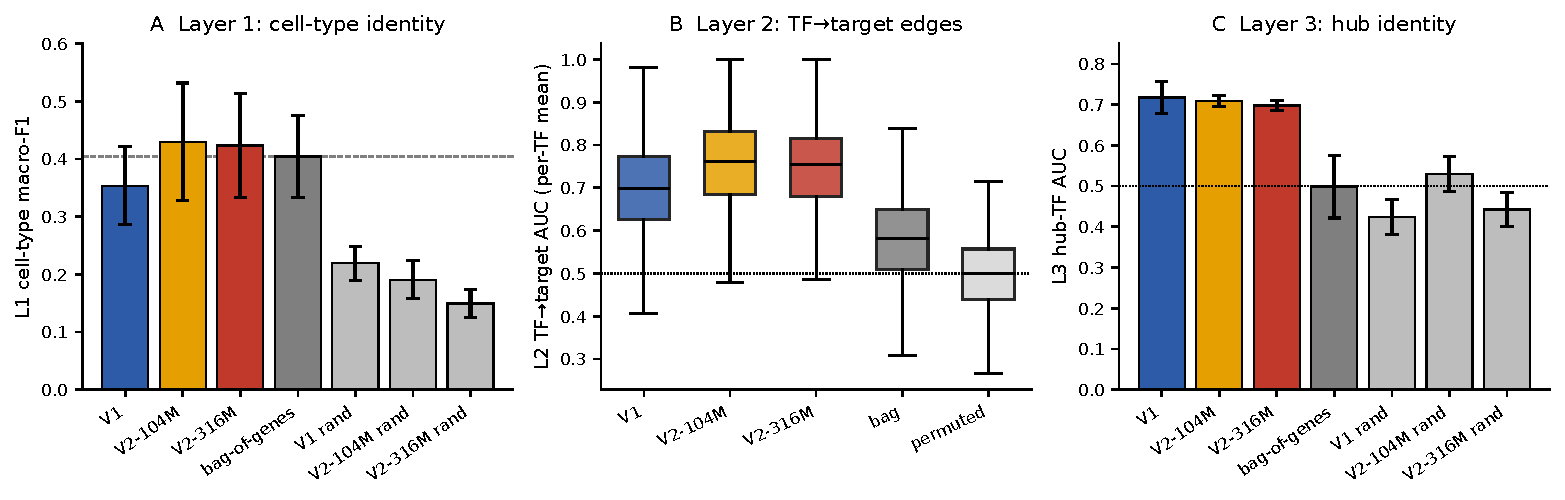
\includegraphics[width=\linewidth]{../results/figures/v2/fig1.pdf}
\caption{\textbf{Three-scale headline numbers across all three probes.} (A) Layer 1 (cell-type identity) macro-F1 across donor-stratified 5-fold CV; bars show mean across folds with 95\% bootstrap CI. (B) Layer 2 (TF$\to$target) per-TF AUC distribution; boxes show median and IQR over 375 TFs. (C) Layer 3 (hub identity) AUC across TF-stratified 5-fold CV. At every panel: trained Geneformer (V1, V2-104M, V2-316M); bag-of-genes baseline; random-init Geneformer at matched architecture/dimension.}
\label{fig:1}
\end{figure}

\begin{figure}[!htbp]
\centering
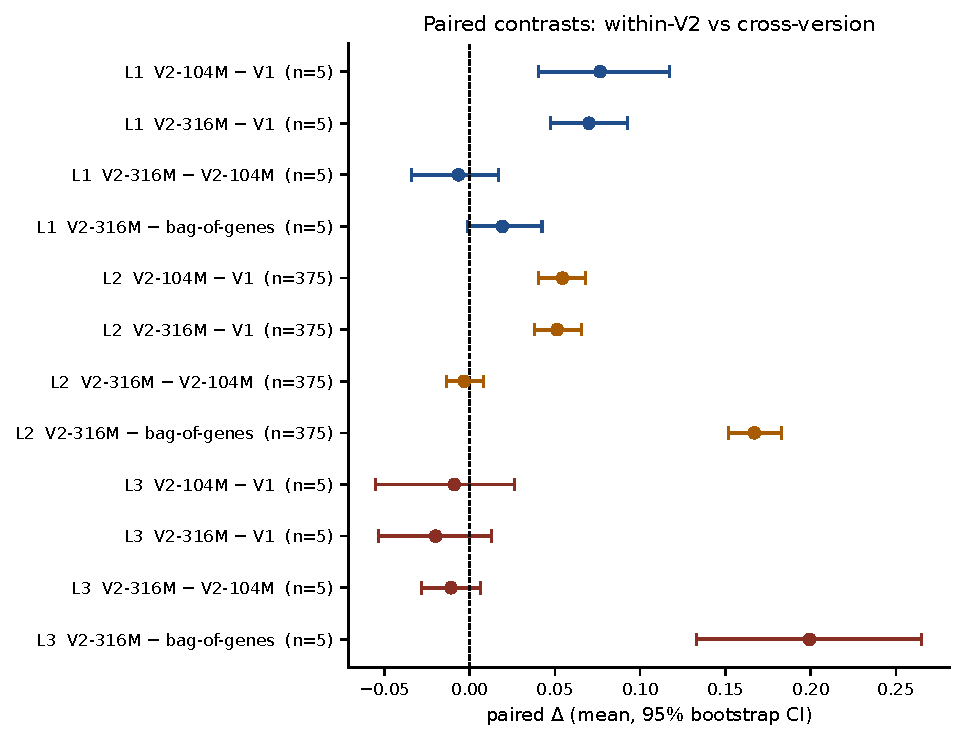
\includegraphics[width=0.85\linewidth]{../results/figures/v2/fig2.pdf}
\caption{\textbf{Forest plot: paired scaling deltas across V1$\to$V2 (confounded) and within V2 (parameter-only).} For each probe, three contrasts: V1$\to$V2-104M, V1$\to$V2-316M, and V2-104M$\to$V2-316M. Within-V2 paired deltas are within noise of zero on every probe; the V1$\to$V2 deltas on L1 and L2 are real but conflate parameter, corpus, and vocabulary changes. Whiskers are 95\% bootstrap CIs.}
\label{fig:2}
\end{figure}

\begin{figure}[!htbp]
\centering
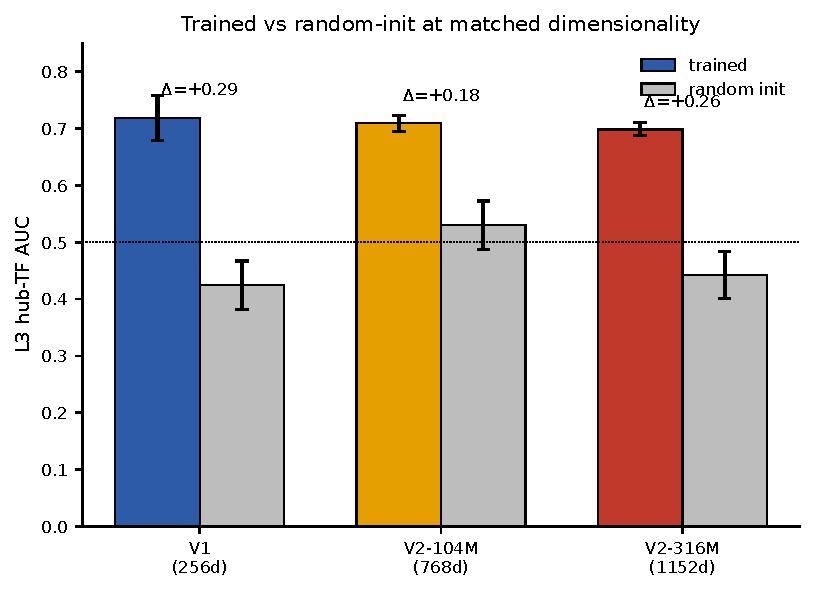
\includegraphics[width=0.85\linewidth]{../results/figures/v2/fig3.pdf}
\caption{\textbf{Geometry-falsifying random-init control across embedding dimensions.} Trained vs.\ random-init L3 hub-AUC at 256-d (V1-10M), 768-d (V2-104M), and 1152-d (V2-316M). The trained-minus-random gap exceeds 0.18 AUC at every dimension, ruling out the alternative that hub identity is recoverable purely from geometric room.}
\label{fig:3}
\end{figure}

\begin{figure}[!htbp]
\centering
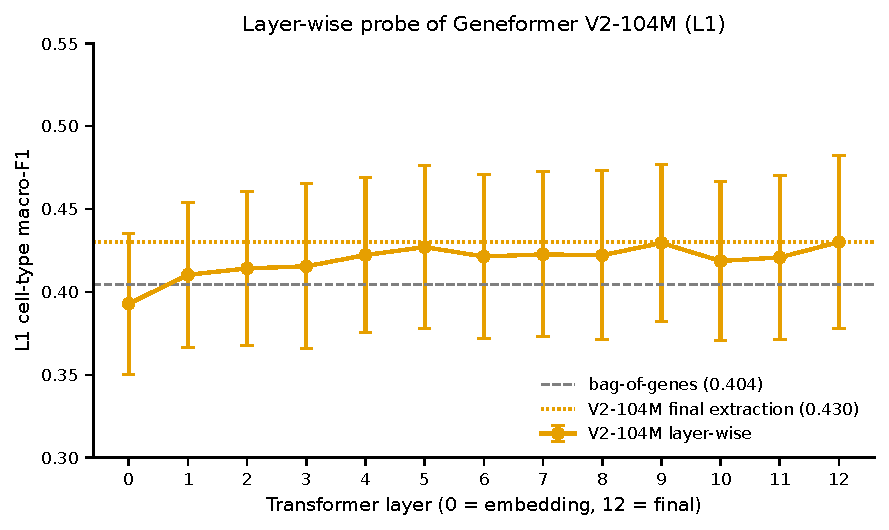
\includegraphics[width=0.85\linewidth]{../results/figures/v2/fig4.pdf}
\caption{\textbf{Layer-wise V2-104M Layer 1 macro-F1.} Cell-type-identity macro-F1 of a fresh linear probe trained on the mean-pooled hidden state at each of the 13 layers (L0 = pre-transformer token embeddings; L1--L12 = transformer blocks). Solid line: mean across 5 donor-stratified folds. Shaded band: $\pm$1 SE. Dashed horizontal line: bag-of-genes baseline (0.404). No intermediate layer crosses the bag-of-genes line; the final layer used in the headline results (0.430) ties for best.}
\label{fig:4}
\end{figure}

\section{Discussion}\label{discussion}

\subsection{What we can conclude}\label{what-we-can-conclude}

Restricting attention to the only clean parameter-scaling axis the
public Geneformer checkpoints offer --- V2-104M $\to$ V2-316M, a 3$\times$ increase
in parameters at fixed pretraining corpus, fixed vocabulary, and (per
the model cards) the same training schedule --- none of our three probes
show a measurable improvement. Cell-type identity moves by $\Delta$=$-$0.007
macro-F1 (CI {[}$-$0.034, +0.017{]}); TF$\to$target structure by $\Delta$=$-$0.003 AUC
(CI {[}$-$0.014, +0.008{]}, p=0.45 over n=375 TFs); hub-TF identity by
$\Delta$=$-$0.011 AUC (CI {[}$-$0.028, +0.007{]}). The combined V1$\to$V2 transition
does deliver large gains on the L2 TF$\to$target probe (+0.054 AUC, p=10$^{-16}$)
and a modest, power-limited gain on L1 cell-type identity (+0.07
macro-F1, n=5, p=0.063), but those gains conflate three changes ---
parameter count, \textasciitilde3.5$\times$ corpus expansion, and a vocabulary
refresh --- and we cannot attribute them to any one factor. The cleanest
positive finding in the paper is L3: hub topology is encoded in the
input gene-token embeddings of V1-10M at AUC 0.72, exceeds bag-of-genes
by +0.20 AUC at every scale, and the gap survives a
random-initialization control at matched embedding dimensionality
(random-init AUC 0.42 at 256d, 0.53 at 768d, 0.44 at 1152d). This rules
out the alternative interpretation that 256-d (or 768-d, or 1152-d)
Euclidean space simply has enough geometric room to separate any small
subset of gene tokens from the rest. Hub identity is real model
knowledge, it is encoded at the smallest variant, and it does not
benefit measurably from 31$\times$ more parameters or \textasciitilde3.5$\times$ more
pretraining data. Within Geneformer, hub identity is a low-complexity
property --- recoverable from co-expression statistics at modest model
capacity --- that saturates immediately.

\subsection{What we cannot
conclude}\label{what-we-cannot-conclude}

Several things we deliberately do not claim. We do not claim that
parameter scaling fails to help scFMs in general; we tested one model
family and one parameter-scaling step, and a null at this specific step
does not generalize. We do not claim to have decomposed the V1$\to$V2 gain
into parameter-vs-data contributions; doing so cleanly would require
checkpoints that hold all-but-one factor constant --- a 10M-parameter
Geneformer trained on the V2 corpus, or a 104M-parameter Geneformer
trained on Genecorpus-30M --- and neither exists in public release. We
do not claim Geneformer ``fails to encode cell-type identity''; the
V1$\to$V2 gain on L1 is real, if power-limited, and the L2 TF$\to$target signal
at V2-316M is large and selectivity-passing. We do not claim hub
identity is generically a low-complexity signal across all single-cell
foundation models; the claim is specifically that \emph{Geneformer}
encodes hub topology above bag-of-genes at every tested scale.
Establishing the same property for scGPT, UCE, scFoundation, or
Nicheformer requires running the L3 probe on those embeddings, which we
did not.

The within-V2 nulls on L1 and L3 are explicitly power-limited. With n=5
paired-fold observations the smallest two-sided Wilcoxon p attainable is
0.063 and our 95\% bootstrap CI on the V2-104M $\to$ V2-316M difference
rules out improvements larger than roughly +0.02 macro-F1 (L1) or +0.01
AUC (L3); smaller effects we cannot detect at this n.~The L2 within-V2
null is on firmer footing --- it pairs across n=375 TFs rather than 5
folds and has a CI that excludes anything larger than +0.008 AUC --- but
the L1 and L3 statements remain ``no measurable improvement at our
power'' rather than ``no improvement.'' The L1 V2-316M-vs-bag-of-genes
comparison ($\Delta$=+0.019, p=0.31) is similarly a failure to reject the null
hypothesis of equality, not a positive demonstration of equivalence; we
did not pre-specify an equivalence margin and did not perform two
one-sided tests, so the careful phrasing throughout this paper is
``fails to exceed'' rather than ``matches'' or ``is equivalent to.''
Finally, our three probes are all linear logistic regression on frozen
embeddings of healthy human blood/immune cells; the signal we find or
fail to find on those probes is silent on what a non-linear probe, a
different tissue, or a fine-tuned classifier would see.

\subsection{Connection to prior
work}\label{connection-to-prior-work}

Our finding that the largest publicly available Geneformer variant fails
to exceed a bag-of-genes baseline on cell-type identity is consistent
with the emerging consensus that scFMs do not reliably beat
raw-expression baselines on tasks they were ostensibly designed to solve
\citep{boiarsky2025}. What we add to that consensus is a controlled three-scale
parameter sweep on a single model family, run with the full Hewitt-Liang
selectivity discipline plus a random-initialization control at matched
dimensionality, plus an explicit decomposition of the V1$\to$V2 transition
into parameter and corpus components. The selectivity-passing positive
findings we do report (L3 hub identity at every scale, L2 TF$\to$target at
V2 scale) are stronger than the typical scFM benchmark precisely because
of those controls.

The Theodoris-group scaling paper \citep{venkatesh2026} reports monotonic accuracy improvements with
Geneformer scale on fine-tuned classifiers. Our null on within-V2
parameter scaling for frozen-embedding linear probes is not in conflict
with that result. Fine-tuning lets the model rewrite its representation
and frozen probing does not, and the two regimes can scale differently.
The most direct reading consistent with both findings is that the
Venkatesh et al.~gains arise during fine-tuning rather than being
available off-the-shelf in the pretrained representation --- which is a
meaningful distinction for any practitioner deciding whether to deploy
V2-316M frozen embeddings as features in a downstream pipeline. Civale
et al.~(2026, \emph{arXiv preprint}) recently showed that intermediate
transformer layers can substantially outperform final-layer pooling for
trajectory and perturbation tasks in scFoundation and Tahoe-X1. We use
final-layer mean-pool \citep{reimers2019sbert} throughout the headline
numbers; layer-wise probing on V2-104M for our L1 cell-identity probe is
robust to layer choice (no intermediate layer beats final-layer
mean-pool on macro-F1). The Civale-style layer-wise gain may exist for
our L2 or L3 probes --- that is open.

\subsection{What the field should take
away}\label{what-the-field-should-take-away}

The most actionable observation from this study, for users of
Geneformer's published checkpoints, is that the apparent gain ``from
scale'' between V1 and V2 is concentrated in the corpus-expansion and
vocabulary-refresh axes, not in the parameter axis. Pure parameter
scaling within the V2 family --- 3$\times$ more parameters at fixed data ---
does not measurably improve any of our three frozen-embedding probes.
This is the single-cell analog of the Chinchilla observation \citep{hoffmann2022chinchilla} that for compute-optimal training, parameter count and
training tokens should scale jointly, and that scaling parameters at
fixed data is the wrong axis to push. Practitioners selecting between
V2-104M and V2-316M as a frozen feature extractor should expect roughly
equivalent performance on the kinds of probes we ran, and should weigh
the 3$\times$ inference-cost difference accordingly. Practitioners considering
whether to push for a hypothetical V3 with more parameters at the same
\textasciitilde104M-cell corpus should expect, by the same logic,
diminishing returns on frozen embeddings; the more productive next axis
is data, not parameters. Our results say nothing about the
parameter-vs-data trade-off for fine-tuned downstream classifiers, where
the \citet{venkatesh2026} result is the more relevant precedent.

A second, more general takeaway concerns probing methodology. The
selectivity control \citep{hewitt2019} and the random-initialization
control \citep{zhang2018random} cost almost nothing to run --- a
re-execution of the same probe with permuted labels and an
untrained-but-same-architecture model --- and they substantively change
what one is allowed to claim. Random initialization at V1's 256-d alone
produces an L3 hub-AUC of 0.42 and at V2-316M's 1152-d an AUC of 0.44;
without the matched-dimensionality random-init control, an unsuspecting
reader could read our L3 result as ``linear separability of any small
class in 1000-d Euclidean space'' rather than as model knowledge. We
urge that future scFM benchmarking adopt the
selectivity-plus-random-init pair as a default, not an optional add-on.

\subsection{Future work}\label{future-work}

Four extensions seem most useful. First, systematic layer-wise probing
of Geneformer for the L2 TF$\to$target and L3 hub-identity probes --- the
\citet{civale2026} result that intermediate layers carry task-relevant
signal that final-layer pooling discards is established for other scFMs
and other tasks, and our L1 layer-wise null does not generalize
automatically to gene-relational probes. Second, replication of all
three probes on scGPT, UCE, and scFoundation. The L3 hub claim in
particular needs cross-model evidence before it can be promoted from
``Geneformer encodes hub topology'' to ``scFMs encode hub topology.''
Third, cross-tissue generalization. Healthy human blood/immune is a
single tissue with strong cell-type structure and a deep regulatory
literature; whether the same probes report the same scaling patterns on
brain, gut, or tumor tissue is unknown. Fourth --- and this is a request
to model trainers more than a research direction --- a Geneformer
checkpoint suite that holds all-but-one factor constant (a 10M-parameter
Geneformer on the V2 corpus, or a 104M-parameter Geneformer on
Genecorpus-30M) would let the field cleanly decompose the V1$\to$V2 confound
that we and the Theodoris group are currently both unable to resolve.
Until such a suite exists, scaling claims for scFMs that compare across
model-family transitions will continue to confound parameter count with
corpus and vocabulary change, and any single-axis interpretation of
those comparisons will rest on assumption rather than evidence.

\section{Reproducibility}\label{reproducibility}

Code, environment, and data-pull scripts are committed at
\url{https://github.com/williamcolegithub/Morpheus} (made public concurrent with this preprint release) and archived at Zenodo, concept DOI \href{https://doi.org/10.5281/zenodo.20046043}{10.5281/zenodo.20046043} (always resolves to the latest version; the version snapshot accompanying this preprint is \texttt{v1.0-preprint}, DOI \href{https://doi.org/10.5281/zenodo.20046044}{10.5281/zenodo.20046044}, 6 May 2026). Pinned \texttt{uv.lock};
deterministic seed \texttt{0} threaded through every random component.
Census release 2025-11-08; \texttt{decoupler} 2.1.6;
\texttt{transformers} 4.57; PyTorch 2.11.0+mps (laptop, current PyPI
release at extraction time) and PyTorch 2.5.1+cu124 (AWS EC2; the cloud
CUDA 12.4 driver predates the cu130-built 2.11 wheels, so we pinned the
cloud env to 2.5.1+cu124 — the only library version that differs across
laptop and cloud, and it does not affect any numerical result). Pipeline reproduces end-to-end on a 24 GB MacBook Air (V1)
plus two AWS EC2 g5.xlarge sessions (V2-104M and V2-316M,
\textasciitilde\$5 each). Full per-fold and per-TF results are released
as parquet files; figures are regenerable via
\texttt{morpheus.analysis.figures\_v2}.

\section*{Data availability}

All data used in this work are publicly available from existing repositories. The single-cell expression corpus is the human blood/immune subset of the CZ CELLxGENE Census release 2025-11-08, accessed via the \texttt{cellxgene\_census} Python package \citep{cellxgene2025}. Transcription-factor regulons are DoRothEA confidence levels A/B/C \citep{garciaalonso2019dorothea} and CollecTRI \citep{mullerdott2023collectri}, both accessed via \texttt{decoupler} \citep{badiaimompel2022decoupler}. Pretrained Geneformer model weights and gene-vocabulary dictionaries are distributed at \url{https://huggingface.co/ctheodoris/Geneformer} \citep{theodoris2023}. The exact data-pull scripts used to fetch and preprocess these resources are committed in the project repository (see Code availability).

\section*{Code availability}

The full reproducible pipeline --- data acquisition, embedding extraction, probe runners, sensitivity sweep, statistics, and figure generation --- is committed at \url{https://github.com/williamcolegithub/Morpheus} under the MIT License, and archived at Zenodo with concept DOI \href{https://doi.org/10.5281/zenodo.20046043}{10.5281/zenodo.20046043} (the v1.0-preprint snapshot accompanying this manuscript is at DOI \href{https://doi.org/10.5281/zenodo.20046044}{10.5281/zenodo.20046044}). All per-fold and per-TF results, the stats summary, the bibliography, and the figure-generation source are included.

\section*{Acknowledgments}

The author thanks the developers of the open-source resources this work depends on: the CZ CELLxGENE team for the Census infrastructure; the Saez-Rodriguez group for DoRothEA, CollecTRI, and \texttt{decoupler}; the Theodoris group for releasing Geneformer weights, vocabulary dictionaries, and rank-value tokenization code; and the maintainers of \texttt{scanpy}, \texttt{anndata}, \texttt{scikit-learn}, \texttt{transformers}, and PyTorch. Compute for V2-104M and V2-316M extractions was self-funded on AWS EC2.

\paragraph{AI assistance.} The author used large language model assistants (Anthropic Claude) for code drafting, manuscript editing, and adversarial review during preparation. All scientific design, experimental execution, statistical analysis, and final interpretive judgments are the author's; the author takes full responsibility for the manuscript's scientific content.

\section*{Competing interests}

The author declares no competing interests.

\section*{Funding}

This work received no external funding. Compute and infrastructure costs were self-funded.

\bibliographystyle{plainnat}
\bibliography{references}

\end{document}
